\documentclass{article}

% to compile a camera-ready version, add the [final] option, e.g.:
% \usepackage[final]{nips_2016}

%!TEX root = main.tex
%%%%%%%%%%%%%%%%%%%%%%%%%%%%%%%%%%%%%%%%%%%%%%%%%%%%%%%%%%%%%%%%%%%%%%%%%%%%%%%%%%%%
\usepackage[utf8]{inputenc} % allow utf-8 input
\usepackage[T1]{fontenc}    % use 8-bit T1 fonts
\usepackage{hyperref}       % hyperlinks
\usepackage{url}            % simple URL typesetting
\usepackage{booktabs}       % professional-quality tables
\usepackage{amsfonts}       % blackboard math symbols
\usepackage{nicefrac}       % compact symbols for 1/2, etc.
\usepackage{microtype,natbib}   

\usepackage{times,bbm,amsthm,comment,amssymb,amsmath,amsfonts, mathtools, hhline, enumerate}

\usepackage{graphicx} % more modern
\usepackage{subfigure} 
\usepackage{algorithm}
\usepackage{algorithmic}

\mathtoolsset{
showonlyrefs=true%true % or false in draft mode
}

\newcommand{\DBA}[1]{{\bf\color{red} [DBA: #1]}}
\newcommand{\NPD}[1]{{\bf\color{red} [NPD: #1]}}
\newcommand{\MDR}[1]{{\bf\color{red} [MKR: #1]}}
\newcommand{\RCW}[1]{{\bf\color{red} [RCW: #1]}}


\DeclareMathOperator*{\argmax}{argmax}
\DeclareMathOperator*{\argmin}{argmin}
\DeclareMathOperator*{\argsup}{argsup}
\DeclareMathOperator*{\arginf}{arginf}
\DeclareMathOperator*{\diag}{diag}

\DeclareMathOperator*{\expec}{\mathbb E}
\DeclareMathOperator*{\exphat}{\hat{\mathbf E}}
\newcommand{\indic}{{\mathbbm 1}}

\newcommand{\chosen}{{\texttt{Chosen}}}
\newcommand{\actual}{{\texttt{Actual}}}
\newcommand{\comply}{{\texttt{Comply}}}

\newcommand{\x}{{\mathbf x}}
\newcommand{\y}{{\mathbf y}}
\newcommand{\wt}{{\mathbf w}}
\newcommand{\vt}{{\mathbf v}}
\newcommand{\bp}{{\mathbf p}}
\newcommand{\bP}{{\mathbf P}}
\newcommand{\bt}{{\mathbf b}}
\newcommand{\be}{{\mathbf e}}
\newcommand{\cA}{{\mathcal A}}
\newcommand{\cB}{{\mathcal B}}
\newcommand{\cC}{{\mathcal C}}
\newcommand{\cH}{{\mathcal H}}
\newcommand{\cR}{{\mathcal R}}
\newcommand{\bR}{{\mathbb R}}

\newcommand{\fN}{{\mathfrak N}}
\newcommand{\fC}{{\mathfrak C}}
\newcommand{\fA}{{\mathfrak A}}
\newcommand{\fD}{{\mathfrak D}}


\newcommand{\grad}{\operatorname{\nabla}}
\newcommand{\dd}{{\partial}}

\newcommand{\prob}{{\mathbb P}}
\newcommand{\probq}{{\mathbb Q}}

\newcommand{\eod}{{${}$\\}}

\newcommand{\regret}{{\mathtt{Regret}}}
\newcommand{\proj}{{\mathtt{Proj}}}

\newcommand*\loss{\ensuremath{\boldsymbol\ell}}
\newcommand*\Loss{\ensuremath{\mathcal L}}
\newcommand*\error{\mathcal E}


\newtheorem{thm}{Theorem}
\newtheorem{cor}{Corollary}
\newtheorem{prop}{Proposition}
\newtheorem{lem}{Lemma}
\newtheorem{eg}{Example}
\newtheorem{defn}{Definition}
\newtheorem{assn}{Assumption}
\newtheorem{claim}[thm]{Claim}
\theoremstyle{remark}
\newtheorem*{idea}{Proof idea}
\newtheorem*{rem}{Remark}
\newtheorem{ex}{Exercise}
\newtheorem*{qu}{Question}
\newtheorem{challenge}{Challenge}



\title{
Compliance-Aware Bandits: Improved No-Regret Learning with Applications to Clinical Trials
}

\author{Nicolas Della Penna, Mark D. Reid, David Balduzzi}
\begin{document} 

\maketitle

\begin{abstract} 
	Motivated by clinical trials, we study bandits with observable non-compliance. 
	At each step, the learner chooses an arm, after, instead of observing only the reward, it also observes the action that took place.
	We show that such noncompliance can be helpful or hurtful to the learner in general.
	Unfortunately, naively incorporating compliance information into bandit algorithms loses guarantees on sublinear regret.
	We present hybrid algorithms that maintain regret bounds up to a multiplicative factor and can incorporate compliance information.
	Simulations based on real data from the International Stoke Trial show the practical potential of these algorithms.
\end{abstract} 

%!TEX root = main.tex
%%%%%%%%%%%%%%%%%%%%%%%%%%%%%%%%%%%%%%%%%%%%%%%%%%%%%%%%%%%%%%%%%%%%%%%%%%%%%%%%%%%%%%%%
\section{Introduction}
\label{bandintro}

People often don't do as they are told. Approximately 50\% of patients suffering from chronic illness do not take prescribed medications (\cite{sabate:03}). It is safe to assume that the rate at which patients or doctors will follow the recommendations provided by an algorithm will fall well short of 100\%. 
Unfortunately, despite its importance in medical applications (\cite{vrijens:12,hugtenburg:13}), compliance has not been analyzed in the bandit literature. 

In this chapter, we introduce compliance awareness into the \emph{bandit setting} (\cite{bubeck:12}).
Bandit problems are concerned with optimal repeated decision-making in the presence of uncertainty. The main challenge is to trade-off exploration and exploitation, so as to collect enough samples to estimate the rewards from different strategies whilst also strongly biasing samples towards those actions most likely to yield high rewards.  
Our running example is an algorithm that recommends treatments to patients. For concreteness, consider a mobile app that encourages patients who have recently suffered a stroke to carry out various low intensity interventions that may be beneficial in preventing future strokes.
These could be as simple as meditating, going for a walk or taking an aspirin.
The effects of the interventions on the probability of a future stroke may be small. The social benefits of collectively choosing the most effective interventions, however, may be large.
 
There are other settings in which compliance information is available. For example, an algorithm could recommend treatments to doctors. Whether or not the doctor then prescribes the recommended treatment to the patient is extremely informative, since the doctor may make observations and have access to background knowledge that is not available to the algorithm.
A quite different setting is online advertising, where bandit algorithms are extensively applied to recommend which ad to display (\cite{graepel:10,mcmahan:13}). In practice, the recommendations provided by the bandit may not be followed. For example, sales teams often have hand-written rules that override the bandit in certain situations. Alternatively, the algorithm may assign a user to a treatment on their laptop, and when the user is not logged in, expose him to a different treatment on their mobile.
Clearly, the bandit algorithm should be able to learn more efficiently if it is provided  with information about which ads were actually shown.

In the classic multi-armed bandit setting, the player chooses one of $k$-arms on each round and receives a reward( \cite{auer:02b,auer:02}). The player is not told what the reward would have been had it chosen a different arm. The goal is to minimize the cumulative regret over a series of $T$ rounds. In the more general compliance setting, the action chosen by the algorithm is not necessarily the action that is finally carried out, see section~\ref{sec:formal}. Instead, a compliance process mediates between the algorithm's recommendation and the action that is actually taken. Importantly, the compliance process may depend on latent characteristics of the subject of the decision. We focus on the case where the outcome of the compliance process is observable.

Unfortunately, compliance information is a two-edged sword. There are settings where it is useful; but  it can also lead to linear regret. We present sub-linear regret algorithms that incorporate compliance information and provide both worst case regret guarantees that match up to multiplicative constants the standard ones for multi-armed bandits (which we term the chosen strategy). We also show with stylized examples situations where compliance aware algorithms have bounded regret and standard ones do not.


\subsection{Outline}
Section~\ref{sec:noncompliance} introduces the formal compliance setting and introduces three protocols for incorporating compliance information into bandit algorithms. Each protocol has strengths and weaknesses. The simplest protocol ignores compliance information -- yielding the classical setting where standard regret bounds hold. If, instead of attending to its recommendations, the bandit attends to whether the patient actually takes the treatment, then it is possible to learn faster than without compliance information. On the other hand, there are no guarantees on convergence when an algorithm attends purely to the compliance of patients and ignores its own prior recommendations -- examples of linear regret are provided in section~\ref{sec:protocols}. 

A natural goal is thus to simultaneously incorporate compliance information whilst preserving the no-regret guarantees of the classical setting. We then present two hybrid algorithms that do both. The first, \texttt{HB} is in a two-level bandit algorithm. The bottom-level learns three experts that specialize on difference kinds of compliance information. The top-level is another bandit that learns which expert performs optimally. The algorithm thus has no-regret against both the treatments and two natural reward protocols that incorporate compliance information. The second algorithm, \texttt{TB}, rapidly converges to Thompson sampling with standard guarantees. However, when Thompson sampling is unsure about which arm to pull, the algorithm takes advantage of the uncertainty to introduce arm-pulls sampled from \texttt{HierchicalBandit}.

Empirically, \texttt{TB} achieves a surplus of 8.9 extra survivals (that is, human lives) relative to the randomized baseline.
The \texttt{HB} algorithm with \texttt{Epsilon Greedy} as the base algorithm achieves a surplus of 9.2.
In contrast, the best performing strategy that is not compliance aware is Thompson sampling, which yields 7.9 extra survivals.



\subsection{Comparison with other bandit settings}
It is useful to compare noncompliance with other bandit settings. Partial monitoring is concerned with situations where the player only partial observes its loss \cite{alon:15}. Our setting is an extension of the bandit setting, where additional compliance-information is provided. Whether or not a patient complies is a form of side-information. However, in contrast to the side-information available to contextual bandits, compliance is only observed \emph{after} an arm is pulled. An interesting question, left for future work, is how contextual and compliance information can both be incorporated into bandit algorithms.

Hybrid algorithms were previously proposed in the best-of-both-worlds scenario( \cite{bubeck:12a,seldin:14}), where the goal is to construct a bandit that plays optimally in both stochastic and adversarial environments. Vapnik introduced a related notion of side-information into the supervised setting with his learning under privileged information framework (\cite{vapnik:09}). 
An important point of comparison is the bandits with unobserved confounders model introduced in( \cite{bareinboim:15}). That paper was motivated using an extended example involving two subpopulations (drunk and sober) gambling in a casino. Since we are primarily interested in clinical applications, we map their example onto two subpopulations of patients, rich and poor. Suppose that rich patients always take the treatment (since they can afford it) and that they are also healthier in general. Poor patients only take the treatment when prescribed by a doctor.

In \cite{bareinboim:15}) they observe that the question ``what is the patient's expected reward when taking the treatment (formally: $\expec[R|{A=1}]$)?'' is confounded by the latent variable \texttt{wealth}. Estimating the effect of the treatment -- which may differ between poor and rich patients -- requires more refined questions. In our notation: 
``what is the patient's expected reward when taking the treatment, given she is wealthy (formally: $\expec[R|{A=1}, \text{always-taker}]$)?'' and  ``what is the patient's expected reward when taking the treatment, given she is poor (formally: $\expec[R|{A=1}, \text{complier}]$)'', see example~\ref{eg:rich}.
The solution proposed in (\cite{bareinboim:15}) is based on the regret decision criterion (RDC), which estimates the optimal action according to $\argmax_{a}\expec[R|A=a,\text{patient's inclination}]$, where the action chosen, $A=a$, may \emph{differ} from the patient's latent inclination. Essentially, computing the RDC requires imposing interventions via the $do(\cdot)$ operator. However, overruling a patient or doctor's decision is often impossible and/or unethical in clinical settings. The counterfactual information required to compute the RDC may therefore not be available in practice.
Compliance information does not act as a direct substitute for the $do(\cdot)$ operator. However, compliance information is often readily available and, as we show below, can be used to ameliorate the effect of confounders by giving a partial view into the latent structure of the population that the bandit is interacting with.






%!TEX root = main.tex
%%%%%%%%%%%%%%%%%%%%%%%%%%%%%%%%%%%%%%%%%%%%%%%%%%%%%%%%%%%%%%%%%%%%%%%%%%%%%%%%%%%%%%%%
\section{Model}
\label{sec:noncompliance}

This section introduces a formal setting for bandits with noncompliance and introduces protocols that prescribe how to make use of compliance information. Before diving into the formalism let us discuss, informally, how compliance information can be useful. 

First, suppose that the patient population is homogeneous in their response to the treatment, and that patients take the treatment with probability $p$ if prescribed and probability $1-p$ otherwise where $p<0.5$. In this setting, it is clear that a bandit algorithm will learn faster by rewarding arms according to whether the treatment was \emph{taken} by the patient, rather than whether it was \emph{recommended} to the patient. 

As a second example, consider \emph{corrective compliance} where patients who benefit from a treatment are more likely to take it, since they have access to information that the bandit does not. The bandit clearly benefits by learning from the information expressed in the behavior of the patients. Learning from the treatment actually taken is therefore more efficient than learning from the bandit's recommendations. Further examples are provided in section~\ref{sec:formal}.


%TODO: frame as a partial monitoring games, two armed equivalence ref %http://arxiv.org/pdf/1108.4961v1.pdf 
% Toward a classification of finite partial-monitoring games
% Partial-monitoring games constitute a mathematical framework for sequential decision making problems with imperfect feedback: the learner repeatedly chooses an action, the opponent responds with an outcome, and then the learner suffers a loss and receives a feedback signal, both of which are fixed functions of the action and the outcome. The goal of the learner is to minimize his total cumulative loss. We make progress toward the classification of these games based on their minimax expected regret. Namely, we classify almost all games with two outcomes and a finite number of actions: we show that their minimax expected regret is either zero, , Θ(T2/3), or Θ(T), and we give a simple and efficiently computable classification of these four classes of games. Our hope is that the result can serve as a stepping stone toward classifying all finite partial-monitoring games.


\begin{figure*}[t]
	\centering	
	\begin{tikzpicture}[scale=2, transform shape]
% nodes %
\node[text centered] (a) {$a$};
\node[left = 1.5 of a, text centered] (c) {$c$};
\node[right=1.5 of a, text centered] (r) {$r$};
\node[draw, rectangle, dashed, above = 1 of a, text centered] (u) {$u$};
 
% edges %
\draw[->, line width= 1] (c) --  (a);
\draw [->, line width= 1] (a) -- (r);
%\draw[->,red, line width= 1,dashed] (u) --node {X} (c);
\draw[->,line width= 1] (u) --(r);
\draw[->,line width= 1] (u) -- (a);
%\draw[->, red, line width=1,dashed] (c) to  [out=270,in=270, looseness=0.5] node{X} (r);
\end{tikzpicture}

	\caption{Bandit with Compliance Awareness DAG}
\end{figure*}


%%%%%%%%%%%%%%%%%%%%%%%%%%%%%%%%%%%%%%%%%%%%%%%%%%%%%%%%%%%%%%%%%%%%%%%%%%%%%%%%%%%%%%%%
\subsection{Formal setting}
\label{sec:formal}

We consider a sequential decision making problem where a process mediates between the actions chosen by the algorithm and the action carried out in the world. The general game is as follows:

\begin{defn}[bandit with compliance information]\label{def:compliance_bandit}\eod
	At each time-step $t$, the player selects an action $c_t\in \cA=[k]=\{1,\ldots,k\}$ (the chosen action). The environment responds by carrying out an action $a_t\in\cA=[k]$ (the actual action) and providing reward $r_t\in[0,1]$, or loss $\ell_t$.

	The standard bandit setting is when $a_t$ is either unobserved or $c_t = a_t$ for all $t\in[T]$.
\end{defn}
  
Given this model, we define the ``noncompliance level'' $n(c, u)$ for a specific choice $C=c$ and latent variables $U=u$ to mean the probability that $A \neq c$ given those values, that is, $n(c, u) = 1 - P(A=c|C=c, U=u)$.

Compliance and outcomes are often confounded. For example, healthy patients may be less inclined to take a treatment than unhealthy patients. 
The set of compliance-behaviors is the set of functions $\cC=\{\nu:\cA\rightarrow\cA\}$ from advice to treatment-taken \cite{koller:09}. 

\begin{defn}[model assumptions]\label{def:assumptions}\eod
	We make the following assumptions:
	\begin{enumerate}
		\item Compliance $\nu(u)\in\cC$ depends on a latent variable sampled i.i.d. from unknown  $\bP(u)$.
		\item Outcomes $r(\nu(u), a,u)$ depend on compliance-behavior, treatment-taken and the latent $u$. That is, outcomes are a fixed function $r:\cC\times \cA\times U\rightarrow[0,1]$.		
	\end{enumerate}
\end{defn}

The confounding of compliance with outcomes is modeled with a latent variable $u$ such that compliance $\nu(u)$ depends on $u$; and outcomes $r(c,\nu(u),u)$ is a function $r:\cA\times (\cA\rightarrow \cA)\times U\rightarrow [0,1]$ that depends on treatment-advice, compliance and the latent variable $u$.

When $|\cA|=k=2$ (control and treatment), we can list the compliance-behaviors explicitly.
\begin{defn}[compliance behaviors]\label{def:compliance_model}\eod
	For $k=2$, the following four subpopulations capture all deterministic compliance-behaviors:
	\begin{align}
		\text{never-takers ($\fN)$:}     \Big(c_0\mapsto a_0, c_1\mapsto a_0\Big)
		\qquad
		& \text{always-takers ($\fA)$:}    \Big(c_0\mapsto a_1, c_1\mapsto a_1\Big)
		\\
		\text{compliers ($\fC)$:} \Big( c_0\mapsto a_0, c_1\mapsto a_1\Big)
		\qquad
		&\text{defiers ($\fD)$:}    \Big(c_0\mapsto a_1 c_1\mapsto a_0\Big)
	\end{align}
	Let $p_s:= \expec_{u\sim \bP(u)}[\indic_{[\nu(u)=s]}]$ denote the probability of sampling from subpopulation $s\in\{\fN,\fA,\fC, \fD\}$.
\end{defn}
Unfortunately, the subpopulations cannot be distinguished from observations. For example, a patient that takes a prescribed treatment may be a complier or an always-taker. Nevertheless, observing compliance-behavior provides potentially useful side-information. The setting differs from contextual bandits because the side-information is only available \emph{after} the bandit chooses an arm. 	


\begin{defn}[stochastic reward model]\label{def:reward_model}\eod
	The expected reward given subpopulation $s$ and the actual treatment $j\in\cA$ is
	\begin{equation}
		r_{s,j} 
		:= \expec_{u\sim \bP(u)}\big[r(\nu(u),a_j,u)\,\big|\, \nu(u)=s\big]
		\quad\text{for }s\in \{\fN, \fA,\fC,\fD\}.
		\label{eq:exp_rew}		
	\end{equation}		
\end{defn}
The goal is to maximize the cumulative reward received,
i.e. choose a sequence of actions $(c_t)_{t\in T}$ that maximizes $\expec_{u\sim \bP(u)}\left[\sum_t r(\nu(u),\nu(u)(c_t), u)\right]$. We quantify the performance of algorithms in terms of regret, which compares the cumulative reward against that of the best action in hindsight.



%%%%%%%%%%%%%%%%%%%%%%%%%%%%%%%%%%%%%%%%%%%%%%%%%%%%%%%%%%%%%%%%%%%%%%%%%%%%%%%%%%%%%%%%
\subsection{Reward protocols}
\label{sec:protocols}

Since compliance-information is only available after-pulling an arm, it cannot be used directly when selecting arms. However, how compliance-information can be used to modify the updates performed by the algorithm. For example, if the bandit recommends taking a treatment, and the patient does not do so, we have a choice about whether to update the arm that the bandit recommended (treatment) or the arm that the patient pulled (control).
Each protocol can be combined with any multi-armed bandit algorithm. 

\begin{defn}[reward protocols]\label{def:protocols}\eod
	We consider three protocols for assigning rewards to arms:
	\begin{enumerate}[P1.]
		\item \textbf{\chosen: chosen-treatment updates.}
		Assign reward $r_t$ to arm $j$ if $c_t=j$.
		\item \textbf{\actual: actual-treatment updates.}
		Assign reward $r_t$ to arm $j$ if $a_t=j$.
		\item \textbf{\comply: compliance-based updates.}
		Assign reward $r_t$ to arm $j$ if $c_t=j$ and $a_t=j$.
	\end{enumerate}
\end{defn}
The protocols rewards are summarized in the table bellow. Each protocol has strengths and weaknesses.

\subsection{Rewards assigned to arms by the three protocols}
\label{sec:protocol_table}

The rewards assigned to each arm by the three protocols are summarized in the table below. None of the protocols successfully isolates the compliers. It follows, as seen above, that which protocol is optimal depends on the structure of the population, which is unknown to the learner. The table can be extended with additional reward protocols. Here we restrict attention to the three most intuitive protocols.


\begin{center}
\begin{tabular}{| l | c | c | c |}
\hline
Arm updated & \chosen & \actual & \comply \\
\hline
      & $r_{\fN,0}$ & $r_{\fN,0}$ & $r_{\fN,0}$ \\
$i=0$ & $r_{\fC,0}$ & $r_{\fC,0}$ & $r_{\fC,0}$ \\
      & $r_{\fA,1}$ &             &             \\
      & $r_{\fD,1}$ & $r_{\fD,0}$ &             \\
\hline
      & $r_{\fN,0}$ &             &             \\
$i=1$ & $r_{\fC,1}$ & $r_{\fC,1}$ & $r_{\fC,1}$ \\
      & $r_{\fA,1}$ & $r_{\fA,1}$ & $r_{\fA,1}$ \\
      & $r_{\fD,0}$ & $r_{\fD,1}$ &             \\
\hline
\end{tabular}
\end{center}





\paragraph{Protocol \#1: \chosen.}
Under \chosen, the bandit advises the patient on which treatment to take, and ignores whether or not the patient complies. 

\begin{prop}\label{prop:chosen}
	Standard regret bounds hold for any algorithm under \chosen.
\end{prop}


\paragraph{Protocol \#2: \actual.} 
Expected rewards depend on the treatment Eq.~\eqref{eq:exp_rew} chosen by the patient, and not directly on the arm pulled by the bandit. Thus, a natural alternative to \chosen\, is \actual, where the bandit assigns rewards to the treatment that the patient actually used -- which may not in general coincide with the arm that the bandit pulled.

\begin{prop}\label{prop:actual}
	There are settings where \actual\, outperforms \chosen\, and \comply.
\end{prop}
\begin{proof}
	Suppose that $r_{s,j}=r_j$ depends on the treatment but not the subpopulation. Further suppose the population is a mix of always-takers, never-takers, and compliers -- but no defiers. 
	Always-takers and never-takers ignore the bandit, which therefore only interacts with the compliers. 

	The rewards used to update \chosen\, are, in expectation 
	\begin{equation}
		\expec[R\,|\,c_0] 
		= (1-p_\fA)\cdot r_0 + p_\fA\cdot r_1
	\end{equation} and 
	\begin{equation}
		\expec[R\,|\,c_1]
		= p_\fN\cdot r_0 + (1-p_\fN)\cdot r_1
	\end{equation}
	whereas the rewards used to update \actual\, are $\expec[R\,|\,a_0] = r_0$ and $\expec[R\,|\,a_1] = r_1$.
	It follows that
	\begin{equation}
		r_{\fC,0} = \expec[R\,|\,a_0] \neq \expec[R\,|\,c_0] 
	\end{equation} and 
	\begin{equation}
		r_{\fC,1} = \expec[R\,|\,a_1] \neq \expec[R\,|\,c_1].
	\end{equation}
	Thus, \actual\, assigns rewards to arms based on their effect on compliers (which are the only subpopulation interacting with the bandit), whereas the rewards assigned to arms by \chosen\, are diluted by patients who do not take the treatment. Finally, \actual\, outperforms \comply\, because it updates more frequently.
\end{proof}

However, \actual\, can fail completely.
\begin{eg}[\actual\, has linear regret; defiers]\label{eg:defiers}\eod
	Suppose that the population consists in defiers and further suppose the treatment has a positive effect: $r_{\fD,0}=0$ and $r_{\fD,1}=1$.
	Bandit algorithms using protocol \#2 will learn to pull arm $c_1$, causing defiers to pull arm $0$. The best move in hindsight is the opposite.
\end{eg}
Defiers are arguably a pathological case. The next scenario is more realistic in clinical trials:
\begin{eg}[Linear regret; harmful treatment]\label{eg:rich}\eod
	Suppose there are two sub-populations: the first consists of rich, healthy patients who always take the treatment. The second consists of poor, less healthy patients who only take the treatment if prescribed. Finally, suppose the treatment \emph{reduces} well-being by $0.25$ on some metric. We then have
	\begin{equation}
	    \expec[R|a_0] = p_\fC \cdot r_{\fC,0} = 0p_\fC 
	\end{equation} and 
	
	\begin{equation}
	    \expec[R|a_1] = p_\fC \cdot r_{\fC,1} + p_\fA\cdot r_{\fA,1}
	    = -0.25p_\fC + 0.75p_\fA
	\end{equation}
	If the population of healthy always-takers $p_\fA$ is sufficiently large, then \actual\, assigns higher rewards to the \emph{harmful} treatment arm.
\end{eg}


\paragraph{Protocol \#3: \comply.}
Finally, \chosen\, and \actual\, can be combined to form \comply, which only rewards an arm if (i) it was chosen by the bandit and (ii) the patient followed the bandit's advice.

\begin{prop}\label{prop:comply}
	There are settings where \comply\, outperforms \chosen\, and \actual.
\end{prop}

\begin{proof}
	It is easy to see that \comply\, outperforms \chosen\, in the setting of Proposition~\ref{prop:actual}.
	
	Consider a population of never-takers, always-takers and compliers. Suppose that never-takers are healthier than compliers $r_{\fN,0}> r_{\fC,0/1}$ whereas always-takers are less healthy $r_{\fA,1}<r_{\fC,0/1}$.  
    The expected rewards received by \chosen\, are
	\begin{align}
		\expec[R\,|\,c_0]
		& = p_{\fC}r_{\fC,0} + p_\fN r_{\fN,0} + p_\fA r_{\fA,1}
		\\
		\expec[R\,|\,c_1]
		& = p_{\fC}r_{\fC,1} + p_\fN r_{\fN,0} + p_\fA r_{\fA,1}
	\end{align}
	
	Let $q_0$ and $q_1$ be the probability that the bandit pulls arms 0 and 1 respectively. The expected rewards received by \actual\, are
	\begin{equation}
		\expec[R\,|\,a_0]
		 = \frac{q_0 p_{\fC}r_{\fC,0} + p_\fN r_{\fN,0}}{q_0p_\fC + p_\fN}		
		\expec[R\,|\,a_1]
		\quad\text{and}\quad
		 = \frac{p_\fA r_{\fA,1} + q_1p_\fC r_{\fC,1}}{p_\fA + q_1 p_\fC}
	\end{equation}
	whereas the rewards used to update \comply\, are
	\begin{align}
		\expec[R\,|\,c_0,a_0] = \frac{p_{\fC}r_{\fC,0} + p_\fN r_{\fN,0}}{p_\fC + p_\fN}
		\quad\text{and}\quad
		\expec[R\,|\,c_1,a_1] = \frac{p_\fA r_{\fA,1} + p_{\fC}r_{\fC,1}}{p_\fA + p_\fC}
	\end{align}
	It follows that $r_{\fC,0} \leq\expec[R\,|\,c_0,a_0]\leq \expec[R\,|\,a_0]$ and $r_{\fC,} \geq\expec[R\,|\,c_1,a_1] \geq \expec[R\,|\,a_1]$.
	The reward estimates for compliers are diluted under both \texttt{Actual} and \texttt{Comply}. However, \comply's estimate is more accurate.
\end{proof}

It is easy to see that \comply\, also has unbounded regret on example~\ref{eg:rich}.


%%%%%%%%%%%%%%%%%%%%%%%%%%%%%%%%%%%%%%%%%%%%%%%%%%%%%%%%%%%%%%%%%%%%%%%%%%%%%%%%%%%%%%%%

\input{algo.tex}
%%!TEX root = main.tex

%!TEX root = main.tex

\section{Introduction}

The previous chapter introduced a pair of new algorithms that incorporated compliance information and proved that they preserved the worst case performance guarantees up to multiplicative factors.
This leaves open the question as to whether these new algorithms can in fact outperform their standard counterparts in practical settings. 
This chapter uses simulations based on both synthetic and real data from a clinical trial, to asses that.

We first consider simulations based on data from a clinical trial. Given that there is a single suitable dataset, and to explore settings were the data generating process is exactly known, we also consider several stylized models of patient compliance and simulate them.

The full source code and electronic versions of the simulation results can be found at \url{https://github.com/nikete/thesis/blob/master/Simulations.ipynb} .

%%%%%%%%%%%%%%%%%%%%%%%%%%%%%%%%%%%%%%%%%%%%%%%%%%%%%%%%%%%%%%%%%%%%%%%%%%%%%%%%%%%%%%%%
\section{International Stroke Trial Simulation}
\label{sec:data}

The simulation data is taken from The International Stroke Trial (IST) database. A randomized trial where patients believed to have acute ischemic stroke are treated with: aspirin, subcutaneous heparin, both, or neither (\cite{ist:97}).
Complete compliance and mortality data at 14 days for each of 19,422 patients
To the best of our knowledge, this is the only publicly available clinical trial with compliance data that is suitable for simulations of compliance aware algorithms.

An extensive search failed to find other suitable open randomized clinical trials datasets that included compliance. A systematic review by  (\cite{ebrahim:14}) identified only 37 reanalyses of patient-level data from previously published randomized control trials; only five were performed by entirely independent authors.
Data from drug abuse clinical trials is used in (\cite{kuleshov:14}). However, non-compliance is coded as failure so this source, and drug dependence treatments more generally, cannot be used in our setting.  

Given there is substantial loss of follow up at the 6 month measure we focus on the 14 day outcome.


\subsection{Construction of Actual Actions from Compliance Variables}
The main sources of non-compliance in the dataset are: the initial event not a stroke, clinical decision, administration problem, missed out more than 3 doses. A detailed table and counts of these are included in the datasets open access article ( \cite{ist:11}). 
While these might initially seem like reasons to discard the patients from the dataset, non-compliance is not necessarily random. Discarding these patients could cause algorithms to have unbounded regret (since the loss we care about is over all patients). In particular, misdiagnoses, administrative problems, not taking doses and other sources of noncompliance can be confounded with a patient's socio-economic status, age, and overall health. 

To construct our ``actual arm'' variable, we assume that non-compliance entails taking the opposite treatment.
This is well-defined in the Aspirin case, which only has two arms, and thus non-compliance with placebo is likely to be taking the treatment.
Assigning an actual arm pulled in the heparin part of the trial is less clear cut, as it has three arms: none, low and medium. We construct the actual arm variable by combining assignment and non-compliance. Non-compliance with respect to low and medium assigned treatments is coded as  not-takers, while non-compliance by a patient prescribed ``none'' is coded as low.


\subsection{Results}

\begin{figure}
\begin{center}
	%\textwidth, angle=90
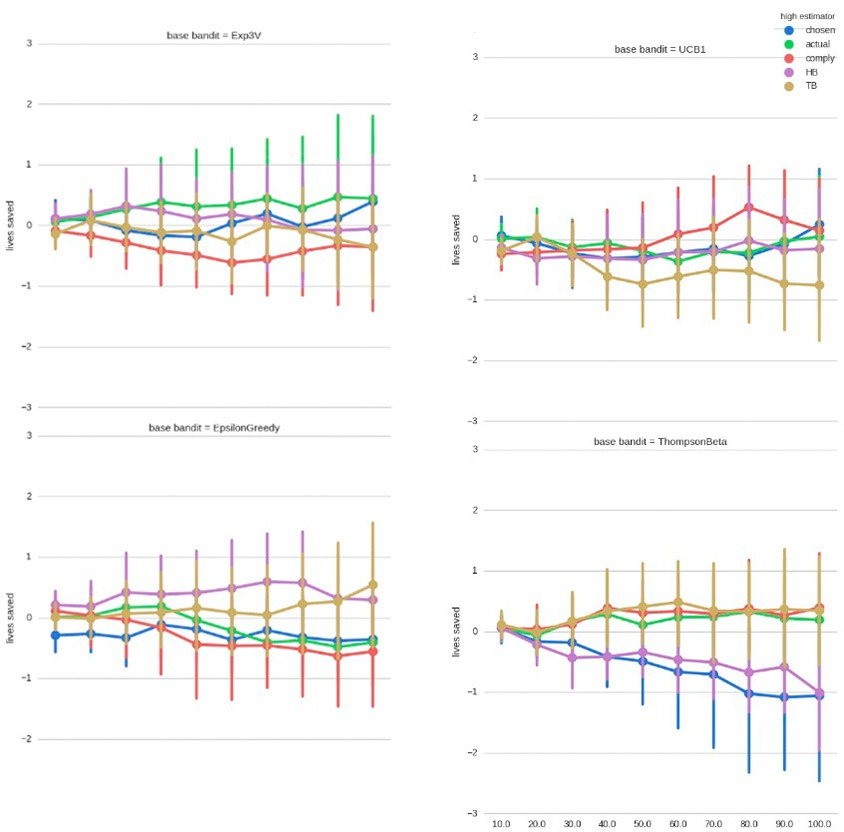
\includegraphics[width=1\columnwidth]{bandit/figs/fig1a.jpeg}
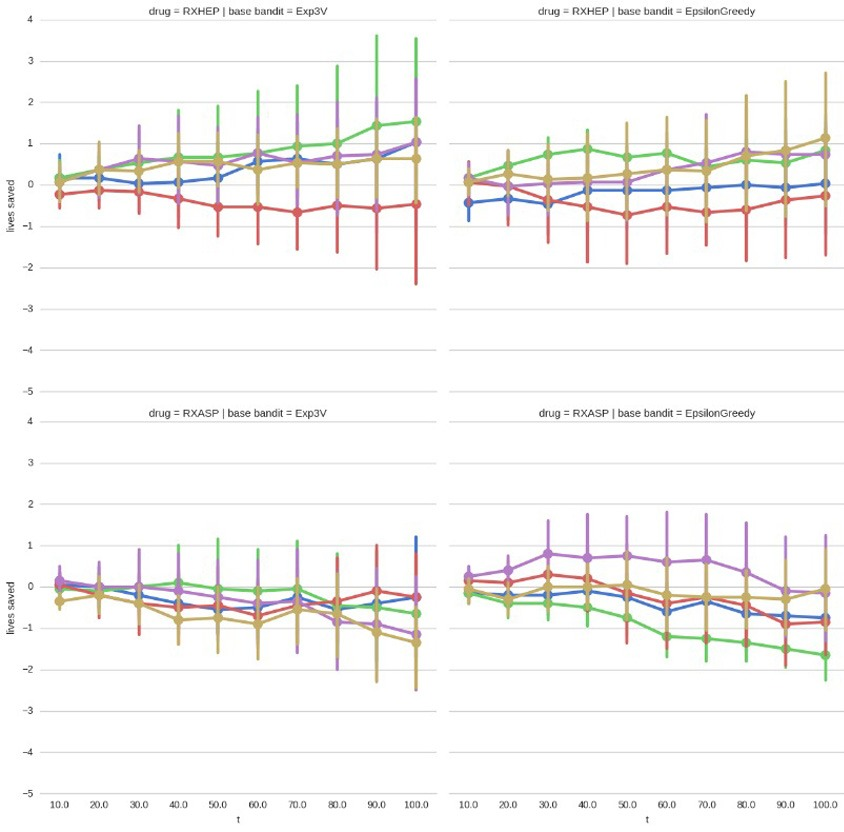
\includegraphics[width=1\columnwidth]{bandit/figs/fig1b.jpeg}
\caption{\textbf{14 Day survivals:} average lives saved over uniform random policy per 10,000 patients in simulated trials of Aspirin and Heparin.}
\label{fig1}
\end{center}
\end{figure} 

We simulated 10,000 patients per run, which allowed us to not oversample the data in any single simulation; 2000 runs were performed, all algorithms were tested against the same draw of the run to minimize unnecessary sampling variation. 

The \texttt{EXP3} gamma parameter was set ahead of time to 0.085, a choice determined by the regret-bounds for $T=10000$ and $K=2$ or $3$. Epsilon-Greedy used a standard annealing schedule. No data dependent parameter tuning was used.
The simulation was carried out by creating a ``counter-factual patient'' by sampling (i.i.d.) one patient from each of the treatment and control groups in the clinical trial. If the algorithm selected the treatment, it then receives the reward and observes the action taken by the subject sampled form the treatment group, and vice versa for the control.


Empirically, \texttt{TB} achieved a surplus of 8.9 extra survivals (that is, human lives) with 95\% confidence interval $[8.1,9.7]$, relative to the randomized baseline.
\texttt{HB} with \texttt{Epsilon Greedy} as the base algorithm achieved a surplus of 9.2 (CI: $[8.3,10.0]$)
In contrast, the best performing strategy that was not compliance aware was Thompson sampling, which yielded 7.9 extra survivals (CI: $[7.2,8.7]$). 

The gains were largely concentrated in the Aspirin trial, which is consistent with the lack of benefits or severe ill effects found in the original study \cite{ist:97} for heparin, and with the small but beneficial effect found for aspirin. 
If the underlying treatment has no positive or negative effect, side-information after the fact alone cannot be helpful.
Note that \actual, and to a lesser extent \comply, performed better than either \chosen\, or the hybrid algorithms. However, these are problematic be used directly since no guarantees apply, their worst case performance unbounc. The performance of the hybrids benefits from the information encoded in \actual\, and \comply\, whilst keeping the guarantees of \chosen. 


A striking secondary finding is the strong interaction between the learning algorithm and the nature of the feedback used. In particular our naive implementation of \texttt{EXP3} performed extremely badly under both \actual\, and \comply, in both the aspirin and heparin simulations. As a result, it is remarkable is that \texttt{EXP3} performs well when used as a top-level algorithm in \texttt{HB} in both trials, and other algorithms on the same data with the same protocol are able to learn better than chosen, while \texttt{EXP3} does worse than random (note the \texttt{EXP3} guarantees are only for the \chosen\, protocol, so do not apply here).



\section{Synthetic Data}


To better understand the behavior of the algorithms in a more varied range of settings, we present results of simulations with synthetic data.
The first simulation illustrates example~2. For comparison, $T$ is kept at 10,000, and we simulated the binary outcome case. We assigned half the patients to rich and half to poor randomly. Rich patients always take the treatment and their outcome, which would otherwise be 1 with $p=1$, becomes 1 with  $p=0.75$. Poor patients only take the treatment when prescribed, their favorable outcome has probability $p=0.5$ without treatment; taking the treatment reduces the probability of a favourable outcome to $p=0.25$. Fig.~2 shows that the performance of \actual\, and \comply\, is much worse than \chosen\, and the hybrid algorithms.



\subsection{Selection of treatment on correlated unobservables}

Consider a harmful treatment. Suppose there are two sub-populations with equal numbers of each. The first consists of rich, healthy patients who always take the treatment. The second consists of poor, less healthy patients who only take the treatment if prescribed. Finally, suppose the treatment reduces survival by 0.25. Assume that the right patients, if they didn't take the treatment would all do well (receive reward of 1), but they all take it, so face only a 0.75 chance of survival. Poor patients who face a baseline survival of 0.75, only take the treatment if instructed, which brings them down from 0.5. Results are for 100 samples.

%\begin{tabular}{llrrrrrlrrrrrl}
\toprule
   &               &   surplus &         &        &        &             &                        &     t &        &       &        &              &                   \\
   &               &      mean &  median &   amin &   amax &         std &                     ci &  mean & median &  amin &   amax &          std &                ci \\
\midrule
HB & EpsilonGreedy &           &         &        &        &             &                        &       &        &       &        &              &                   \\
   & Exp3V &  174.1895 &  153.00 & -263.5 &  533.5 &  147.946788 &    (165.219, 183.2735) &  5500 &   5500 &  1000 &  10000 &  2873.718542 &  (5329.0, 5679.0) \\
   & ThompsonBeta &  142.0385 &  119.75 & -474.0 &  524.0 &  155.149882 &    (132.3765, 151.801) &  5500 &   5500 &  1000 &  10000 &  2873.718542 &  (5324.0, 5678.0) \\
   & UCB1 &  185.5045 &  169.75 & -380.5 &  634.5 &  169.553899 &    (174.9045, 195.937) &  5500 &   5500 &  1000 &  10000 &  2873.718542 &  (5320.0, 5679.0) \\
TB & EpsilonGreedy &  164.1275 &  137.75 &  -92.5 &  526.5 &  126.324350 &   (156.5355, 172.1095) &  5500 &   5500 &  1000 &  10000 &  2873.718542 &  (5323.0, 5675.0) \\
   & Exp3V &  289.3035 &  298.50 & -668.0 &  680.5 &  214.914664 &    (275.9625, 302.343) &  5500 &   5500 &  1000 &  10000 &  2873.718542 &  (5321.0, 5680.0) \\
   & ThompsonBeta &  297.4625 &  303.75 & -678.5 &  698.5 &  207.917822 &   (284.0285, 310.1175) &  5500 &   5500 &  1000 &  10000 &  2873.718542 &  (5325.0, 5677.0) \\
   & UCB1 &  306.1865 &  312.00 & -631.0 &  699.5 &  202.821630 &   (293.4995, 318.3395) &  5500 &   5500 &  1000 &  10000 &  2873.718542 &  (5321.0, 5678.0) \\
actual & EpsilonGreedy &  312.8985 &  312.50 & -602.0 &  676.5 &  197.493261 &     (300.614, 325.125) &  5500 &   5500 &  1000 &  10000 &  2873.718542 &  (5317.0, 5672.0) \\
   & Exp3V & -267.7995 & -260.00 & -614.5 &    0.0 &  153.773319 &    (-277.54, -258.495) &  5500 &   5500 &  1000 &  10000 &  2873.718542 &  (5318.0, 5678.0) \\
   & ThompsonBeta & -315.3935 & -311.25 & -675.5 &  -19.5 &  180.209696 &  (-326.0585, -303.666) &  5500 &   5500 &  1000 &  10000 &  2873.718542 &  (5321.0, 5672.0) \\
   & UCB1 & -228.9745 & -213.75 & -642.0 &   13.0 &  141.402885 &  (-237.771, -220.2625) &  5500 &   5500 &  1000 &  10000 &  2873.718542 &  (5318.0, 5674.0) \\
chosen & EpsilonGreedy &  -79.1915 &  -66.75 & -308.0 &   54.5 &   71.682714 &      (-83.738, -74.79) &  5500 &   5500 &  1000 &  10000 &  2873.718542 &  (5321.0, 5672.0) \\
   & Exp3V &  294.8915 &  292.25 &  -38.5 &  616.5 &  161.242274 &    (284.8325, 304.806) &  5500 &   5500 &  1000 &  10000 &  2873.718542 &  (5320.0, 5681.0) \\
   & ThompsonBeta &  249.8975 &  238.75 & -151.0 &  615.5 &  169.257902 &    (239.5855, 260.232) &  5500 &   5500 &  1000 &  10000 &  2873.718542 &  (5325.0, 5681.0) \\
   & UCB1 &  328.8535 &  327.25 & -118.5 &  687.5 &  181.694511 &   (317.5725, 340.0625) &  5500 &   5500 &  1000 &  10000 &  2873.718542 &  (5322.0, 5681.0) \\
comply & EpsilonGreedy &  284.2595 &  278.75 &   19.5 &  625.5 &  166.451764 &   (273.7875, 294.4835) &  5500 &   5500 &  1000 &  10000 &  2873.718542 &  (5326.0, 5671.0) \\
   & Exp3V &  -48.2795 &  -70.00 & -600.5 &  574.0 &  292.451920 &     (-66.124, -29.997) &  5500 &   5500 &  1000 &  10000 &  2873.718542 &  (5320.0, 5682.0) \\
   & ThompsonBeta & -290.8165 & -281.00 & -643.5 &  262.5 &  182.486686 &   (-302.0395, -279.63) &  5500 &   5500 &  1000 &  10000 &  2873.718542 &  (5318.0, 5672.0) \\
   & UCB1 &   -6.7395 &   -7.50 & -672.5 &  590.5 &  228.589111 &       (-20.708, 7.563) &  5500 &   5500 &  1000 &  10000 &  2873.718542 &  (5320.0, 5672.0) \\
\bottomrule
\end{tabular}


%\begin{tabular}{llrrrrrlrrrrrl}
\toprule
   &               &   surplus &         &        &        &             &                        &     t &        &       &        &              &                   \\
   &               &      mean &  median &   amin &   amax &         std &                     ci &  mean & median &  amin &   amax &          std &                ci \\
\midrule
HB & EpsilonGreedy &           &         &        &        &             &                        &       &        &       &        &              &                   \\
   & Exp3V &  174.1895 &  153.00 & -263.5 &  533.5 &  147.946788 &    (165.219, 183.2735) &  5500 &   5500 &  1000 &  10000 &  2873.718542 &  (5329.0, 5679.0) \\
   & ThompsonBeta &  142.0385 &  119.75 & -474.0 &  524.0 &  155.149882 &    (132.3765, 151.801) &  5500 &   5500 &  1000 &  10000 &  2873.718542 &  (5324.0, 5678.0) \\
   & UCB1 &  185.5045 &  169.75 & -380.5 &  634.5 &  169.553899 &    (174.9045, 195.937) &  5500 &   5500 &  1000 &  10000 &  2873.718542 &  (5320.0, 5679.0) \\
TB & EpsilonGreedy &  164.1275 &  137.75 &  -92.5 &  526.5 &  126.324350 &   (156.5355, 172.1095) &  5500 &   5500 &  1000 &  10000 &  2873.718542 &  (5323.0, 5675.0) \\
   & Exp3V &  289.3035 &  298.50 & -668.0 &  680.5 &  214.914664 &    (275.9625, 302.343) &  5500 &   5500 &  1000 &  10000 &  2873.718542 &  (5321.0, 5680.0) \\
   & ThompsonBeta &  297.4625 &  303.75 & -678.5 &  698.5 &  207.917822 &   (284.0285, 310.1175) &  5500 &   5500 &  1000 &  10000 &  2873.718542 &  (5325.0, 5677.0) \\
   & UCB1 &  306.1865 &  312.00 & -631.0 &  699.5 &  202.821630 &   (293.4995, 318.3395) &  5500 &   5500 &  1000 &  10000 &  2873.718542 &  (5321.0, 5678.0) \\
actual & EpsilonGreedy &  312.8985 &  312.50 & -602.0 &  676.5 &  197.493261 &     (300.614, 325.125) &  5500 &   5500 &  1000 &  10000 &  2873.718542 &  (5317.0, 5672.0) \\
   & Exp3V & -267.7995 & -260.00 & -614.5 &    0.0 &  153.773319 &    (-277.54, -258.495) &  5500 &   5500 &  1000 &  10000 &  2873.718542 &  (5318.0, 5678.0) \\
   & ThompsonBeta & -315.3935 & -311.25 & -675.5 &  -19.5 &  180.209696 &  (-326.0585, -303.666) &  5500 &   5500 &  1000 &  10000 &  2873.718542 &  (5321.0, 5672.0) \\
   & UCB1 & -228.9745 & -213.75 & -642.0 &   13.0 &  141.402885 &  (-237.771, -220.2625) &  5500 &   5500 &  1000 &  10000 &  2873.718542 &  (5318.0, 5674.0) \\
chosen & EpsilonGreedy &  -79.1915 &  -66.75 & -308.0 &   54.5 &   71.682714 &      (-83.738, -74.79) &  5500 &   5500 &  1000 &  10000 &  2873.718542 &  (5321.0, 5672.0) \\
   & Exp3V &  294.8915 &  292.25 &  -38.5 &  616.5 &  161.242274 &    (284.8325, 304.806) &  5500 &   5500 &  1000 &  10000 &  2873.718542 &  (5320.0, 5681.0) \\
   & ThompsonBeta &  249.8975 &  238.75 & -151.0 &  615.5 &  169.257902 &    (239.5855, 260.232) &  5500 &   5500 &  1000 &  10000 &  2873.718542 &  (5325.0, 5681.0) \\
   & UCB1 &  328.8535 &  327.25 & -118.5 &  687.5 &  181.694511 &   (317.5725, 340.0625) &  5500 &   5500 &  1000 &  10000 &  2873.718542 &  (5322.0, 5681.0) \\
comply & EpsilonGreedy &  284.2595 &  278.75 &   19.5 &  625.5 &  166.451764 &   (273.7875, 294.4835) &  5500 &   5500 &  1000 &  10000 &  2873.718542 &  (5326.0, 5671.0) \\
   & Exp3V &  -48.2795 &  -70.00 & -600.5 &  574.0 &  292.451920 &     (-66.124, -29.997) &  5500 &   5500 &  1000 &  10000 &  2873.718542 &  (5320.0, 5682.0) \\
   & ThompsonBeta & -290.8165 & -281.00 & -643.5 &  262.5 &  182.486686 &   (-302.0395, -279.63) &  5500 &   5500 &  1000 &  10000 &  2873.718542 &  (5318.0, 5672.0) \\
   & UCB1 &   -6.7395 &   -7.50 & -672.5 &  590.5 &  228.589111 &       (-20.708, 7.563) &  5500 &   5500 &  1000 &  10000 &  2873.718542 &  (5320.0, 5672.0) \\
\bottomrule
\end{tabular}



\begin{figure}
	\centering	
	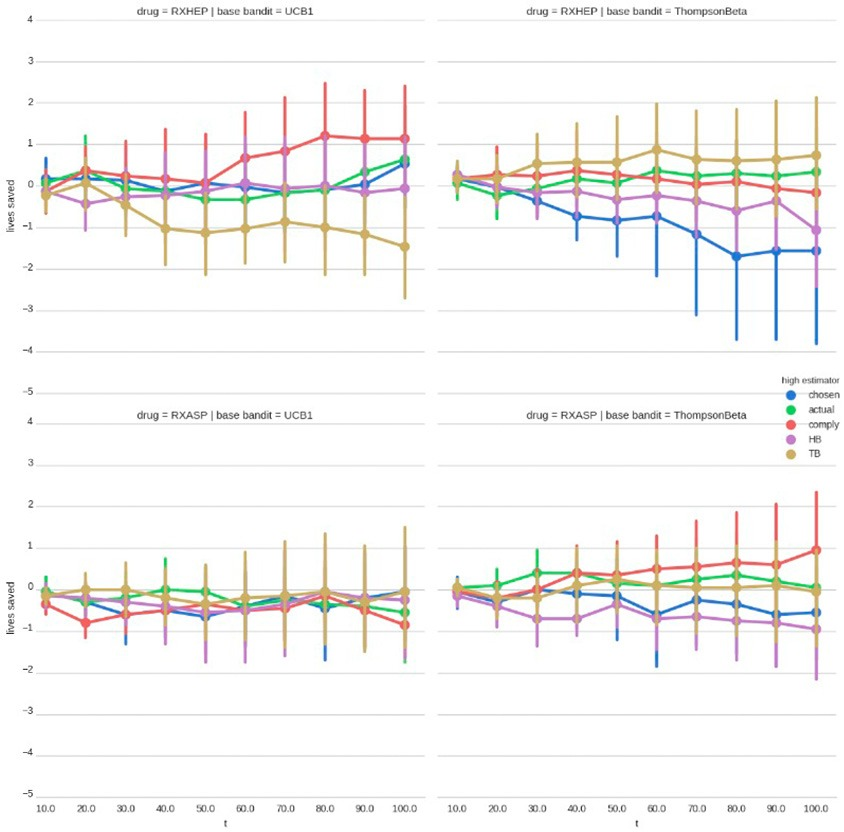
\includegraphics[width=1\columnwidth]{bandit/figs/ex2.jpeg}\hspace{1cm}
	\label{fig:ex2}
	\caption{Worse than random regret across estimators with naive uses of compliance awareness with simulated data from 100 patients sampled from a model of a harmful treatment that is profound by selection into treatment.}
\end{figure}



\subsection{Small T}

The second simulation concerns small $T$. A motivation for very small $T$ adaptive clinical trials is provided by rare diseases. The overall size of the patient population is by construction severely restricted in this setting.  The priors for the mechanisms of action are also often poorly understood, so potential alternative treatments can have radically different probabilities of success. We simulate a $T=12$ adaptive trial with binary outcomes, with two treatments and expected rewards drawn uniformly from the unit interval, and compliance uniformly at random. We sample 1,000 such simulations.
While our bounds are vacuous in this settings, it is interesting that there is on average an  improvement from taking the noncompliance information into account.


\begin{figure}[t]
	\centering	
	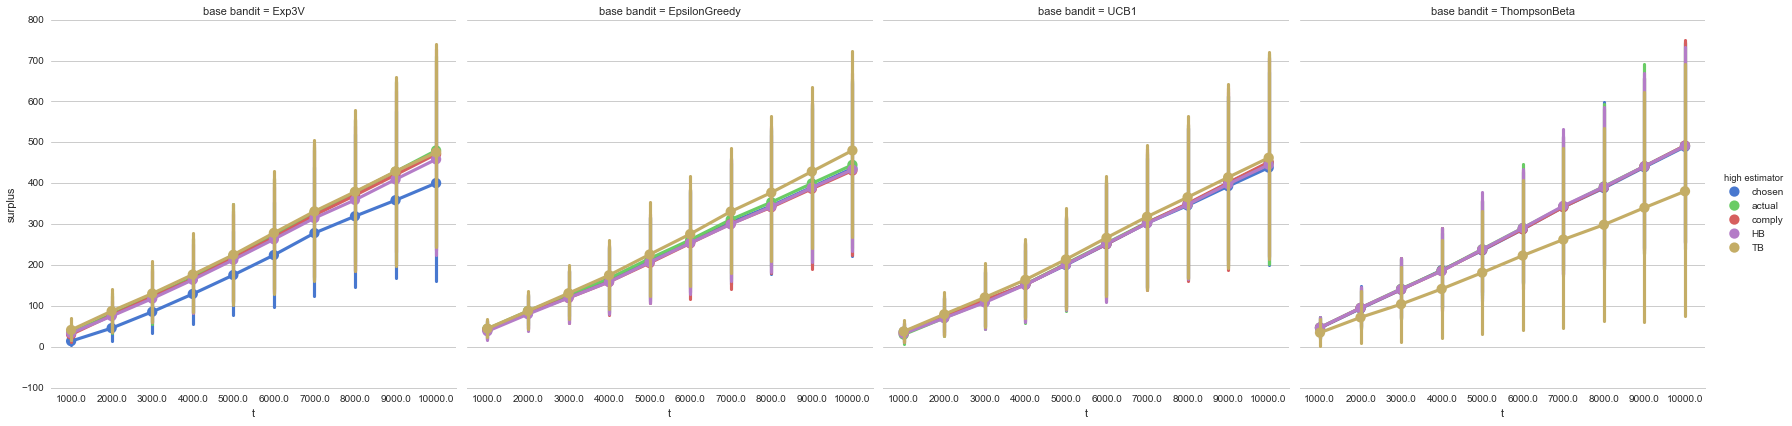
\includegraphics[width=1.5\columnwidth, angle=90]{bandit/figs/ex3.png}\hspace{1cm}
	\label{fig:ex3}
	\caption{12 patients, a not uncommon size of clinical trials in rare diseases or neonatal populations.}
\end{figure}





\subsection{Noncompliance for Best Arm}


A natural scenario for noncompliance and one that offers substantial potential is when the subject is better informed than the algorithm, and realizes they know a better alternative. 
This provides potentially huge practical advantages, specially in situations with very large numbers of a priori low expectation but high variance actions. 
They allow later subjects to benefit from the information that previous subjects bring to the mechanism, while current compliance unaware algorithms not only waste this information but hurt later subjects as it unnecessary raises the apparent variance of the rewards in the arms (since the chosen arm may indeed be very bad relative to the actual arm).




\begin{figure}[t]
	\centering	
	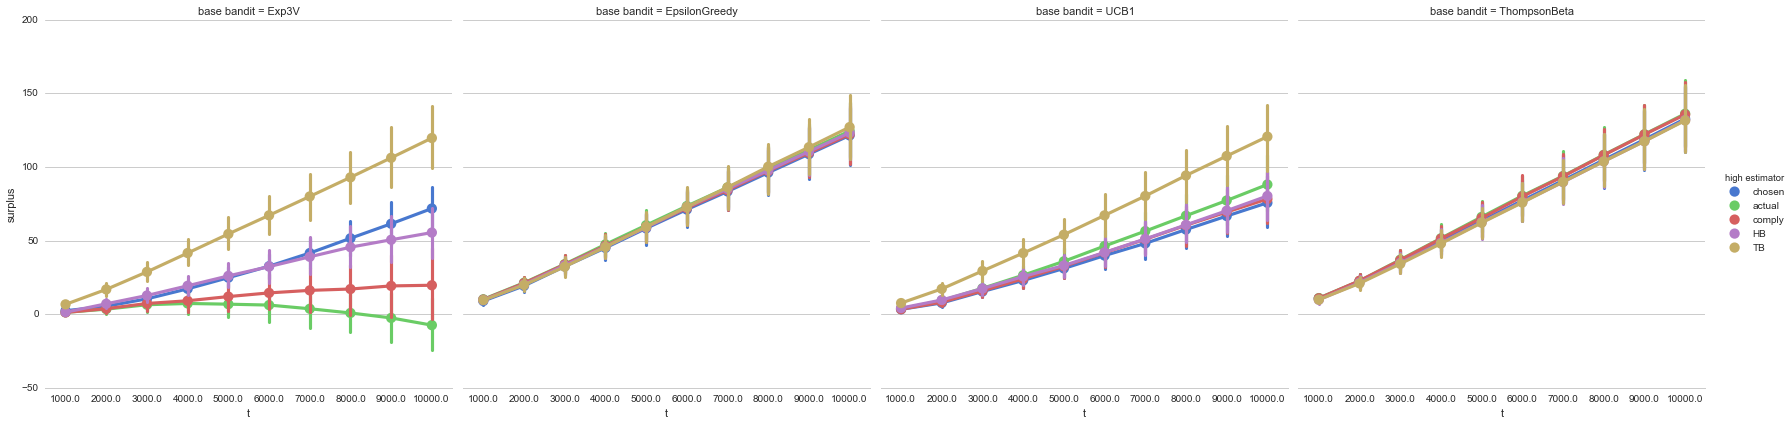
\includegraphics[width=1.5\textwidth, angle=90]{bandit/figs/ex4.png}\hspace{1cm}
	\label{fig:ex4}
	\caption{Noncompliance for best arm}
\end{figure}



%     def __init__(self,foo ):
%         n_arms=2
%         self.arm_value = 0.5+0.25*np.random.random(n_arms)
%         self.n_arms = n_arms
%     def draw_subject(self):
%         prefered_arm = stochastic_argmax(self.arm_value)
%         prefered_reward = random.binomial(1,self.arm_value[prefered_arm])
%         r = []
%         for i in range(self.n_arms):
%             if self.arm_value[i] / self.arm_value[prefered_arm] < random.random(): #informative noncompliance
%                 r.append((prefered_arm,prefered_reward))
%             else:  #compliers 
%                 r.append((i,  random.binomial(1,self.arm_value[i])))
%         return r

% example3= sim( nsim=100, T=10001, DGP=NoncomplianceForBestArm , drug="Better arm")
% display_results(example3.loc[example3['t'] == 10000].drop('t',1))



%\subsection{Independent Noncompliance and Rewards}

%We now simulate a neutral model, where compliance is unrelated to the rewards of the arm.
% #always or never takers. current simulation model is not rich enough for defiers, todo?
% class IndependentNoncomplianceAndRewards():
%     def __init__(self,foo):
%         n_arms=2
%         self.arm_value = 0.9+0.1*np.random.random(int(n_arms))
%         # todo add effect_magnitude=1
%         self.n_arms = n_arms
%     def draw_subject(self):
%         if random.random()<0.9: #compliers 
%             r=[(i, random.binomial(1,self.arm_value[i])) for i in range(self.n_arms)]
%         else:   #always takers
%             actual = categorical_draw(self.arm_value)
%             reward = random.binomial(1,self.arm_value[actual])
%             r= [(actual, reward) for i in range(self.n_arms)]
%         return r

    
% example4= sim( nsim=100, T=10001, DGP=IndependentNoncomplianceAndRewards , drug="example")
% display_results(example4.loc[example4['t'] == 10000].drop('t',1))







%think of the babies http://www.ncbi.nlm.nih.gov/pmc/articles/PMC2778326/



%We have two simulations, one in which noncompliance is independent of everything, and one where noncompliance is towards the higher expectation treatment.

%This is a boring figure, not rue what to say about it.
%%%%%%%%%%%%%%%%%%%%%%%%%%%%%%%%%%%%%%%%%%%%%%%%%%%%%%%%%%%%%%%%%%%%%%%%%%%%%%%%%%%%%%%%
%\subsection{Conclusions}

%Empirically, \texttt{TB} achieves a surplus of 8.9 extra survivals (that is, human lives) and \texttt{HB} achieves 9.2 surplus lives compared with 7.9 for the best classical algorithm. This suggests hybrid algorithms can make a significant difference to clinical outcomes.

% TODO, add note on composability and comparing to relatively well understood baselines. plug and play.


\input{further.tex}


{
\footnotesize
\bibliography{compliance.bib}
\bibliographystyle{abbrv}
}

%\clearpage
%!TEX root = main.tex
%\vspace{5mm}
%\noindent
%{\large{\textbf{Appendix}}}

\setcounter{section}{0}
\setcounter{equation}{0}

\renewcommand{\theequation}{A\arabic{equation}}
\renewcommand{\thesection}{\Alph{section}}
%\renewcommand{\thesubsection}{\Alph{section}.}

\renewcommand{\thethm}{A\arabic{thm}}
\renewcommand{\thedefn}{A\arabic{defn}}
\renewcommand{\theeg}{A\arabic{eg}}

%%%%%%%%%%%%%%%%%%%%%%%%%%%%%%%%%%%%%%%%%%%%%%%%%%%%%%%%%%%%%%%%%%%%%%%%%%%%%%%%%%%%%%%%
\section{Appendix}


%%%%%%%%%%%%%%%%%%%%%%%%%%%%%%%%%%%%%%%%%%%%%%%%%%%%%%%%%%%%%%%%%%%%%%%%%%%%%%%%%%%%%%%%
\subsection{Unobserved confounders.}
\label{sec:confounded}

%\cite{bareinboim:15}: ``The study of unobserved confounders is one of the central themes in the modern literature of causal inference. To appreciate the challenges posed by these confounders, consider the comparison between a randomized clinical trial conducted by the Food and Drug Administration (FDA) versus physicians prescribing drugs in their offices. A key tenet in any FDA trial is the use of randomization for the treatment assignment, which precisely protects against biases that might be introduced by physicians. Specifically, physicians may prescribe Drug A for their wealthier patients who have better nutrition than their less wealthy ones, when unknown to the doctors, the wealthy patients would recover without treatment. On the other hand, physicians may avoid prescribing the expensive Drug A to their less privileged patients, who (again unknown to the doctors) tend to suffer less stable immune systems causing negative reactions to the drug. If a naive estimate of the drug’s causal effect is computed based on physicians' data (obtained through random sampling, but not random assignment), the drug would appear more effective than it is in practice -- a bias that would otherwise be avoided by random assignment. Confounding biases (of variant magnitude) appear in almost any application in which the goal is to learn policies (instead of statistical associations), and the use of randomization of the treatment assignment is one established tool to combat them.''

An important point of comparison is the bandits with unobserved confounders model introduced in \cite{bareinboim:15}. That paper was motivated using an extended example involving two subpopulations (drunk and sober) gambling in a casino. Since we are primarily interested in clinical applications, we map their example onto two subpopulations of patients, rich and poor. Suppose that rich patients always take the treatment (since they can afford it) and that they are also healthier in general. Poor patients only take the treatment when prescribed by a doctor.

Barenboim et al observe that the question ``what is the patient's expected reward when taking the treatment (formally: $\expec[R|{A=1}]$)?'' is confounded by the latent variable \texttt{wealth}. Estimating the effect of the treatment -- which may differ between poor and rich patients -- requires more refined questions. In our notation: 
``what is the patient's expected reward when taking the treatment, given she is wealthy (formally: $\expec[R|{A=1}, \text{always-taker}]$)?'' and  ``what is the patient's expected reward when taking the treatment, given she is poor (formally: $\expec[R|{A=1}, \text{complier}]$)'', see example~\ref{eg:rich}.

The solution proposed in \cite{bareinboim:15} is based on the regret decision criterion (RDC), which estimates the optimal action according to $\argmax_{a}\expec[R|A=a,\text{patient's inclination}]$, where the action chosen, $A=a$, may \emph{differ} from the patient's latent inclination. Essentially, computing the RDC requires imposing interventions via the $do(\cdot)$ operator. However, overruling a patient or doctor's decision is often impossible and/or unethical in clinical settings. The counterfactual information required to compute the RDC may therefore not be available in practice.

Compliance information does not act as a direct substitute for the $do(\cdot)$ operator. However, compliance information is often readily available and, as we show below, can be used to ameliorate the effect of confounders by giving a partial view into the latent structure of the population that the bandit is interacting with.


%We show that intervening via the $do(\cdot)$ operator may not be necessary if compliance information is available. Observing whether or not a patient complies with a treatment-recommendation does not provide direct counterfactual information. However, it does provide partial access to the latent structure of the population that can be exploited, as demonstrated below.







%\cite{bareinboim:15}: ``The study of unobserved confounders is one of the central themes in the modern literature of causal inference. To appreciate the challenges posed by these confounders, consider the comparison between a randomized clinical trial conducted by the Food and Drug Administration (FDA) versus physicians prescribing drugs in their offices. A key tenet in any FDA trial is the use of randomization for the treatment assignment, which precisely protects against biases that might be introduced by physicians. Specifically, physicians may prescribe Drug A for their wealthier patients who have better nutrition than their less wealthy ones, when unknown to the doctors, the wealthy patients would recover without treatment. On the other hand, physicians may avoid prescribing the expensive Drug A to their less privileged patients, who (again unknown to the doctors) tend to suffer less stable immune systems causing negative reactions to the drug. If a naive estimate of the drug’s causal effect is computed based on physicians' data (obtained through random sampling, but not random assignment), the drug would appear more effective than it is in practice -- a bias that would otherwise be avoided by random assignment. Confounding biases (of variant magnitude) appear in almost any application in which the goal is to learn policies (instead of statistical associations), and the use of randomization of the treatment assignment is one established tool to combat them.''

%Confounders and counterfactuals were introduced into the bandit setting in \cite{ortega:10,bareinboim:15}. The latter consider an extended example concerning two subpopulations (drunk and sober patrons) in a casino. Since we are primarily interested in clinical applications, we map their example onto two subpopulations of patients, rich and poor. Suppose that rich patients always take the treatment (since they can afford it) and that they are also healthier in general. Poor patients only take the treatment when prescribed by a doctor.

%Barenboim et al observe that the question ``what is the patient's expected reward when taking the treatment (formally: $\expec[R|{A=1}]$)?'' is confounded by the latent variable \texttt{wealth}. Estimating the treatment-effect -- which may differ between poor and rich patients -- requires more refined questions. In our notation:  ``what is the patient's expected reward when taking the treatment, given she is wealthy (formally: $\expec[R|{A=1}, \text{always-taker}]$)?'' and  ``what is the patient's expected reward when taking the treatment, given she is poor (formally: $\expec[R|{A=1}, \text{complier}]$)''. 

%The solution proposed in \cite{bareinboim:15} is based on the regret decision criterion (RDC), which estimates the optimal action $\argmax_{a}\expec[R|A=a,\text{patient's inclination}]$ where the action chosen may \emph{differ} from the patient's latent inclination. Essentially, an intervention is imposed via a $do(\cdot)$ operator. However, overruling a patient or doctor's decision is often impossible and/or unethical in clinical settings. The counterfactual information required to compute the RDC may therefore not be accessible.

%We show that intervening via the $do(\cdot)$ operator may not be necessary if compliance information is available. Observing whether or not a patient complies with a treatment-recommendation does not provide direct counterfactual information. However, it does provide partial access to the latent structure of the population that can be exploited, as demonstrated below.

%%%%%%%%%%%%%%%%%%%%%%%%%%%%%%%%%%%%%%%%%%%%%%%%%%%%%%%%%%%%%%%%%%%%%%%%%%%%%%%%%%%%%%%%
\subsection{Rewards assigned to arms by the three protocols}
\label{sec:protocol_table}

The rewards assigned to each arm by the three protocols are summarized in the table below. None of the protocols successfully isolates the compliers. It follows, as seen above, that which protocol is optimal depends on the structure of the population, which is unknown to the learner. The table can be extended with additional reward protocols. Here we restrict attention to the three most intuitive protocols.


\begin{center}
\begin{tabular}{| l | c | c | c |}
\hline
Arm updated & \chosen & \actual & \comply \\
\hline
      & $r_{\fN,0}$ & $r_{\fN,0}$ & $r_{\fN,0}$ \\
$i=0$ & $r_{\fC,0}$ & $r_{\fC,0}$ & $r_{\fC,0}$ \\
      & $r_{\fA,1}$ &             &             \\
      & $r_{\fD,1}$ & $r_{\fD,0}$ &             \\
\hline
      & $r_{\fN,0}$ &             &             \\
$i=1$ & $r_{\fC,1}$ & $r_{\fC,1}$ & $r_{\fC,1}$ \\
      & $r_{\fA,1}$ & $r_{\fA,1}$ & $r_{\fA,1}$ \\
      & $r_{\fD,0}$ & $r_{\fD,1}$ &             \\
\hline
\end{tabular}
\end{center}


%%%%%%%%%%%%%%%%%%%%%%%%%%%%%%%%%%%%%%%%%%%%%%%%%%%%%%%%%%%%%%%%%%%%%%%%%%%%%%%%%%%%%%%%
\subsection{No-regret for \texttt{HB}}
\label{sec:bound}

This section shows that constructing a hierarchical bandit with \texttt{EXP3} yields a no-regret algorithm. The result is straightforward; we include it for completeness. A similar result was shown in \cite{chang:05}. 

First, we construct a hierarchical version of \texttt{Hedge}, Algorithm~\ref{alg:meta-hedge}, which is applicable in the full-information setting. On the bottom-level are $M$ instantiations of \texttt{Hedge}. Instantiation $i$, for $i\in[M]$, plays an $N$-dimensional weight vector and receives $N$-dimensional loss vector $\loss^{(t)}_{i}$ on round $t$. We impose the assumption that all instantiations play $N$-vectors for notational convenience. The top-level is another instantiation of \texttt{Hedge}, which plays a weighted combination of the bottom-level instantiations.

\begin{algorithm}[tb]
   \caption{\texttt{Hierarchical Hedge (HHedge)}}
   \label{alg:meta-hedge}
   \begin{algorithmic}   
   	\STATE {\bfseries Input:} $\eta,\rho>0$\\
   	 $v^{(1)}_{i}=1$ for $i\in[M]$;\\ 
   	 $w^{(1)}_{i,j}=1$ for $(i,j)\in[M]\times[N]$
	\FOR{$t=1$ {\bfseries to} $T$}
	\STATE Set $\x^{(t)} \leftarrow \vt^{(t)}/X^{(t)}$ where $X^{(t)} = \sum_{i=1}^M v^{(t)}_{i}$.
	\STATE Set $\y^{(t)}_{i} \leftarrow \wt^{(t)}_{i}/Y^{(t)}_{i}$ where $Y^{(t)}_{i} = \sum_{j=1}^N w^{(t)}_{i,j}$.
	\STATE Receive feedback $\loss^{(t)}\in [0,1]^{M\times N}$ 
	\STATE Incur loss $\sum_{i,j=1}^{M,N} x^{(t)}_{i}\cdot\ell^{(t)}_{i,j}\cdot y^{(t)}_{i,j}$
	\STATE Updates:
	\begin{align}
		v^{(t+1)}_i & \leftarrow v^{(t)}_{i}\cdot \exp\big(-\eta \sum_{j=1}^N\ell^{(t)}_{i,j}\cdot y^{(t)}_{i,j}\big)
		\\
		w^{(t+1)}_{i,j} & \leftarrow w^{(t)}_{i,j}\cdot \exp\big(-\rho\cdot \ell^{(t)}_{i,j}\big)
	\end{align}
   	\ENDFOR
   	\end{algorithmic}
\end{algorithm}

We have the following lemma:

\begin{lem}\label{lem:meta-hedge}
	Introduce compound loss vector $\tilde{\loss}$ with $\tilde{\ell}^{(t)}_i := \sum_j \ell^{(t)}_{i,j}\cdot y^{(t)}_{i,j}$. Then $\rho$ can be chosen in \texttt{HHedge} such that
	\begin{equation}
		\sum_{t=1}^T \langle \x^{(t)},\tilde{\loss}^{(t)}\rangle 
		\leq  \sum_{t=1}^T \tilde{\loss}^{(t)}_i +
		\leq O(\sqrt{T \log M})\quad\forall i.
	\end{equation}
	Moreover, $\rho$ and $\eta$ can be chosen such that, for all $i$,
	\begin{equation}
		\sum_{t,i,j=1}^{T,M,N} x^{(t)}_{i}\ell^{(t)}_{i,j} y^{(t)}_{i,j}
		\leq \sum_{t=1}^T\ell^{(t)}_{i,j}
		+ O(\sqrt{T \log M} + \sqrt{T \log N}).
	\end{equation}
\end{lem}

\begin{proof}
	Apply regret bounds for \texttt{Hedge} twice.
\end{proof}

Lemma~\ref{lem:meta-hedge} says, firstly, that \texttt{HHedge} has bounded regret relative to the bottom-level instantiations and, secondly, that it has bounded regret relative to any of the $M\times N$ experts on the bottom-level.


Algorithm~\ref{alg:meta-exp2} modifies \texttt{HHedge} so that it is suitable for bandit feedback, yielding \texttt{HEXP3}. A corresponding no-regret bound follows immediately:

\begin{lem}\label{lem:meta-exp}
	Define $\tilde{\loss}$ as in Lemma~\ref{lem:meta-hedge}. Then $\rho$ can be chosen in \texttt{HEXP3} such that
	\begin{equation}
		\expec\left[\sum_{t=1}^T\ell_{x^{(t)},y^{(t)}}\right]
		\leq \sum_{t=1}^T \tilde{\ell}^{(t)}_{i}
		+ O(\sqrt{MT\log M})
	\end{equation}
	Moreover, $\rho$ and $\eta$ can be chosen such that
	\begin{equation}
		\expec\left[\sum_{t=1}^{T} \ell^{(t)}_{x^{(t)},y^{(t)}}\right]
		\leq \sum_{t=1}^T\ell^{(t)}_{i,j}
		+ O(\sqrt{TM \log M} + \sqrt{T N\log N})
	\end{equation}
\end{lem}
\begin{proof}
	Follows from Lemma~\ref{lem:meta-hedge} and bounds for \texttt{EXP3}.
\end{proof}

\begin{algorithm}[tb]
   \caption{\texttt{Hierarchical EXP3 (HEXP3)}}
   \label{alg:meta-exp2}
   \begin{algorithmic}   
   \STATE {\bfseries Input:} $\eta,\rho>0$\\
   	 $v^{(1)}_{i}=1$ for $i\in[M]$;\\ 
   	 $w^{(1)}_{i,j}=1$ for $(i,j)\in[M]\times[N]$
	\FOR{$t=1$ {\bfseries to} $T$}
	\STATE Set $\x^{(t)} \leftarrow \vt^{(t)}/X^{(t)}$ where $X^{(t)} = \sum_{i=1}^M v^{(t)}_{i}$.
	\STATE Set $\y^{(t)}_{i} \leftarrow \wt^{(t)}_{i}/Y^{(t)}_{i}$ where $Y^{(t)}_{i} = \sum_{j=1}^N w^{(t)}_{i,j}$.
	\STATE Draw $x^{(t)}\sim \x^{(t)}$ and $y^{(t)}\sim \y^{(t)}_{x^{(t)}}$.
	\STATE Incur loss $\ell^{(t)}_{x^{(t)},y^{(t)}}\in [0,1]$ 
	\STATE Updates:
	\begin{align}
		v^{(t+1)}_i & \leftarrow \begin{cases}
			v^{(t)}_{i}\cdot 
			\exp\big(-\eta\frac{\ell^{(t)}_{i,j}}{x_i}\big) & i=x^{(t)} \\
			v^{(t)}_{i} & \text{else}
		\end{cases}		 
		\\
		w^{(t+1)}_{i,j} & \leftarrow \begin{cases}
			w^{(t)}_{i,j}\cdot \exp\big(-\rho\frac{\ell^{(t)}_{i,j}}{x_iy_{i,j}}\big) 
			& \text{if }(i,j)=(x^{(t)}, y^{(t)}) \\
			w^{(t)}_{i,j} &\text{else}
		\end{cases}
	\end{align}
   	\ENDFOR
   	\end{algorithmic}
\end{algorithm}

\paragraph{Hierarchical Bandit with Thompson sampler base.}
Algorithm~\ref{alg:bts} (\texttt{BTS}) shows how to modify the Thompson sampler for use as a bottom-level algorithm in \texttt{HB}. The modification applies the importance weighting trick: replace $1$ in Thompson sampling with $\tilde{1}=1/p$, where $p$ is the probability that the top-level bandit calls \texttt{BTS} on the given round. 


\begin{algorithm}[tb]
   \caption{\texttt{Base Thompson Sampler (BTS)}}
   \label{alg:bts}
   \begin{algorithmic}
   	\STATE {\bfseries Input:} Probability $p$ that \texttt{BTS} is called by top-bandit\\
   	\STATE Set $\tilde{1}\leftarrow 1/p$
   	 \STATE For each arm $i$ sample $\theta_i\sim\beta(S_i +\tilde{1},F_i +\tilde{1})$
	\STATE Play arm $i^{(t)} := \argmax_i \theta_i$ and observe reward $r^{(t)}$
	\STATE Sample $b$ from Bernoulli with success probability $r^{(t)}$
	\STATE If $b=1$ then $S_i \leftarrow S_i + \tilde{1}$ else $F_i\leftarrow F_i+\tilde{1}$
   	\end{algorithmic}
\end{algorithm}


%%%%%%%%%%%%%%%%%%%%%%%%%%%%%%%%%%%%%%%%%%%%%%%%%%%%%%%%%%%%%%%%%%%%%%%%%%%%%%%%%%%%%%%%
\subsection{Clinical trial data}
\label{sec:data}

The simulation data is taken from The International Stroke Trial (IST) database. A randomised trial where patients believed to have acute ischaemic stroke are treated with: aspirin, subcutaneous heparin, both, or neither \cite{ist:97}.
Complete compliance and mortality data at 14 days for each of 19,422 patients
To the best of our knowledge, this is the largest publicly available clinical trial with compliance data.\footnote{An extensive search failed to find other open randomized clinical trials datasets that included compliance. A systematic review by  \cite{ebrahim:14} identified 37 reanalyses of patient-level data from previously published randomized control trials; five were performed by entirely independent authors.} Data from drug abuse clinical trials is used in \cite{kuleshov:14}. However, noncompliance is coded as failure so this source, and drug dependence treatments more generally, cannot be used in our setting. Given there is substantial loss of follow up at the 6 month measure we focus on the 14 day outcome. 

\paragraph{Compliance variables.}
The main sources of noncompliance in the dataset are: the initial event not a stroke, clinical decision, administration problem, missed out more than 3 doses. A detailed table and counts of these are included in the datasets open access article \cite{ist:11}. 
While these might initially seem like reasons to discard the patients from the dataset, noncompliance is not necessarily random. Discarding these patients could cause algorithms to have unbounded regret (since the loss we care about is over all patients). In particular, misdiagnoses, administrative problems, not taking doses and other sources of noncompliance can be confounded with a patient's socioeconomic status, age, and overall health. 

To construct our ``actual arm'' variable, we assume that noncompliance entails taking the opposite treatment.
This is well-defined in the Aspirin case, which only has two arms, and thus noncompliance with placebo is likely to be taking the treatment.
Assigning an actual arm pulled in the heparin part of the trial is less clear cut, as it has three arms: none, low and medium. We construct the actual arm variable by combining assignment and noncompliance. Noncompliance with respect to low and medium assigned treatments is coded as  not-takers, while noncompliance by a patient prescribed ``none'' is coded as low.



\section{Full simulation results}

The main body of the text focuses on instantiations of our algorithms that employ Thompson sampling as their underlying strategy. We here report results for comparison to Exp3, UCB1 and Epsilon Greedy. 


\begin{figure*}[t]
	\centering	
	\vspace{-6mm}
	\subfigure[]
	{\includegraphics[width=1\textwidth]{figs/example2allbandits.png}\hspace{1cm}
	\label{fig:rich}}
	\subfigure[]
	{\includegraphics[width=1\textwidth]{figs/T12allbandits.png}
	\label{fig:t12}}
	\caption{
	(a) Average surplus rewards relative to random assignment for Example 2 for 1,000 simulations. 
	(b) Average surplus rewards relative to random assignment for an adaptive trial over 12 patients over 1,000 simulations.}
\end{figure*}
\end{document} 




